%====================================================================================================
% ?????
%====================================================================================================
% TCC
%----------------------------------------------------------------------------------------------------
% Autor				: Jasane Schio
% Orientador		: Gedson Faria
% Co-Orientador		: Angelo Darcy
% Instituição 		: UFMS - Universidade Federal do Mato Grosso do Sul
% Departamento		: CPCX - Sistema de Informação
%----------------------------------------------------------------------------------------------------
% Data de criação	: 01 de Outubro de 2015
%====================================================================================================
% NO FUTURO
\chapter{Introdução} \label{Cap:Introducao}
\section{Contexto}
Como uma prova dos crescentes avanços robóticos nas ultimas décadas, em 1997 foi estabelecida a FIRA\cite{FiraHistory}, Federation of International Robot-soccer Association. Com o intuito de promover o desenvolvimento nas àreas de multi-agentes autonomos e cooperação entre robôs, bem como pesquisas e estudos relacionados a mecatrônica, processamento de imagens e robótica\cite{FiraOverview}. O Futebol de Robôs tem sido  uma das principais áreas de foco por ser um domínio complexo, exigindo autonomia do sistema e solução de problemas em tempo real, como dito por Costa\cite{Costa:2000}. 

Porém a maneira como um técnico de futebol passa as informações para seus jogadores em campo, cara à cara, torna-se indisponível no futebol de robôs, já que neste ambiente tais informações precisam ser passadas via comunicação de dados, onde cada um dos robôs se difere do outro por obter um IP único. Para saber qual dos robôs possui cada IP, eles possuem marcadores com duas cores, uma cor designando o time a qual o robô pertence e outra que o identifica de maneira única dentro de sua equipe. A estratégia, de cada equipe, então detecta os marcadores de cor utilizando técnicas de visão computacional e decide a partir da posição dos robôs, qual atitude será tomada em campo.

Acontece que para identificar cada uma das cores é necessário que se faça o que é chamado de calibração. A calibração de cores ocorre para designar o intervalo de valores que corresponde a cada cor naquele determinado momento. Intervalos de cores podem ser pré definidos, no entanto de acordo com a iluminação presente na imagem esses valores tendem a ser alterados, por isso a calibração em cada jogo se faz necessária.
\section{Motivação}
Durante a Competição Latino Americana de Robótica de 2015, tive a oportunidade de participar juntamente com a equipe CEDRO. Foi a minha primeira vez em um evento deste âmbito, e por este motivo fiz algumas observações sobre as equipes e as partidas, a principal foi quanto a calibração de cores. De forma informal, todo jogo possue um \textit{aquecimento} de 20 minutos, onde a maioria das equipes utilizada deste tempo para fazer a calibração de cores. Na equipes que observei, o processo de calibração era feito de forma manual com uma interface muito semelhante ao deselvolvido por Kyle Hounslow\cite{YouTube}. Em algumas equipes, inclusive foi desenvolvido um novo modelo de cores, como é o caso da POTI(UFRN)\cite{Martins:2007}.

Foi estudado o problema da calibração de cores para competição de futebol de robôs categoria Very Small Size Soccer. Onde a calibração de cada uma das cores em campo acaba se tornando um processo exaustivo por ter de ser feito um a um, cerca de 5 minutos para cada cor. Geralmente o tempo de preparo inicial antes de cada jogo é de 20 minutos, tempo que acaba sendo gasto praticamente inteiro no processo de calibração. Se o processo de calibração fosse automatizado, e assim reduzido, haveria mais tempo para ser usado em melhorias técnicas, hardware dos robôs com problemas, melhorias na estratégia de jogo ou resolvendo problema de comunicação.

\section{Objetivos}

Este trabalho tem por objetivo principal automatizar o sistema de identificação de objetos 
coloridos em imagens provenientes de uma câmera em imagens de tempo real, fazendo a calibração dos valores HSV identificando seus limites mínimos e máximos.  
Se fez necessário um sistema para tal finalidade notando-se:

\begin{itemize}
	\item O alto tempo gasto na calibração de intervalo de cores para cada cor disposta em campo, antes dos jogos;
	\item A necessidade um sistema de identificação automática dos objetos em campo;
	\item A falta de um sistema autônomo de registro do valores HSV;
	\item A necessidade de um sistema de definição de intervalos de cores baseando-se nos objetos em campo .
\end{itemize}

Para desenvolver um sistema que supra essas necessidades, foram propostos os seguintes objetivos específicos:

\begin{itemize}
	
	\item Detecção dos objetos em campo de forma automática; 
	\item Estudo de cores para identificação de intervalos de cores dentro da biblioteca OpenCV;
	\item Categorização das cores dos objetos identificados dentro dos intervalos estudados;
	\item Testar o sistema proposto para identificação de cores.
	
	
\end{itemize}

\newpage

\section{Trabalhos Correlatos}
Para o tema específico deste trabalho, calibração de intervalo de cores para times de futebol de robôs da categoria IEEE Very Small Size Soccer, não foram encontrados trabalhos relacionados, porém foram encontrados Team Discription Papers e descrições de sistemas usados pelos times, onde consta sobre o processo de calibração e os métodos usados\cite{Penharbel:2004}\cite{Rosa:2015}\cite{VSSVision}\cite{PenharbelTime}.

\subsection{Calibra}
O Centro Universitário da FEI\cite{PenharbelTime} utiliza em sua equipe Y04 um sistema denominado CALIBRA\cite{Penharbel:2004}. Desenvolvido para sistemas Linux e com Graphical User Interface\cite{Penharbel:2004}, o sistema de calibração possui um módulo chamado de MainWindow, que é responsavel pela configuração de brilho, cor e contraste da imagem adquirida pela câmera e gera um arquivo que é analizado na hora da criação das cores padrão\cite{PenharbelTime}, onde cores-padrão são definidas como intervalos no espaço de cores HSI\cite{PenharbelTime}.
\begin{figure}[H]
	\centering
	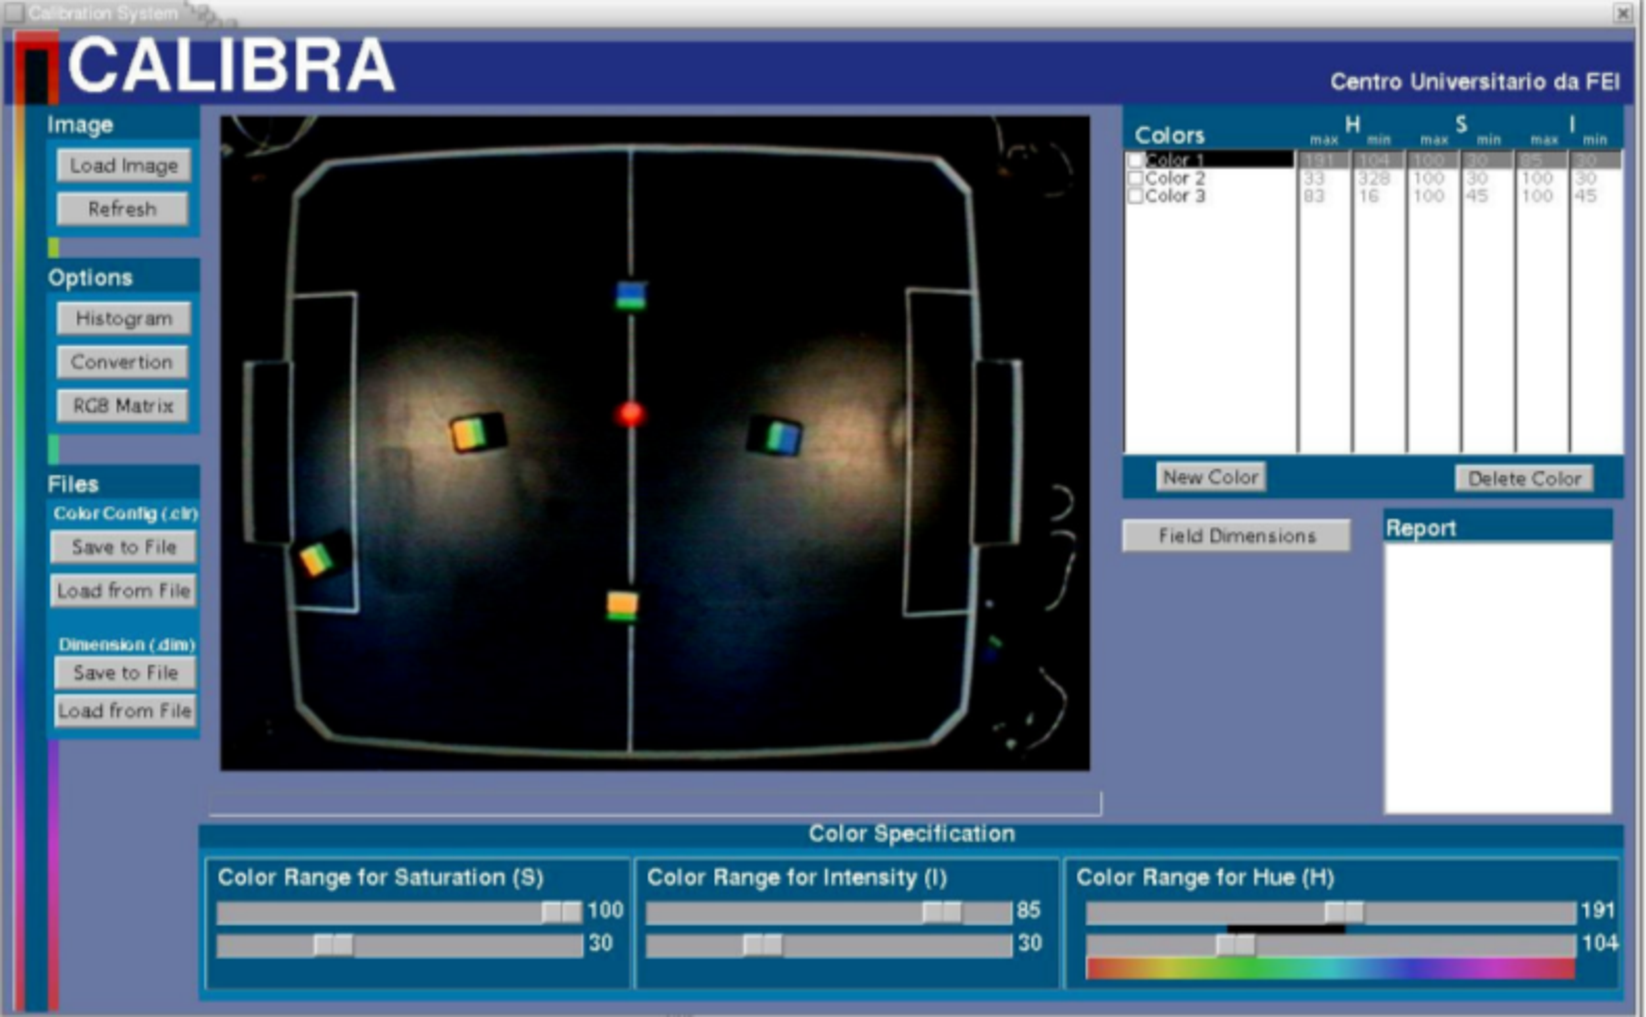
\includegraphics[width=0.6\textwidth]{calibra.pdf}
	\caption{Sistema Calibra desenvolvido pelo Centro Universitário da FEI \cite{Penharbel:2004}}
	\label{Calibra}
\end{figure}

\subsection{VSS-Vision}

Em 2015, Rosa\cite{Rosa:2015} descreveu sobre a equipe de futebol de rob\^os Very Small Size, do Laboratório de Sistemas Inteligentes e Robótica, SIRLab(Faeterj-Petrópolis), o sistema de visão computacional da equipe, durante a competição do ano de 2014, que abrange inclusive a parte de calibração. 

\begin{figure}[H]
	\centering
	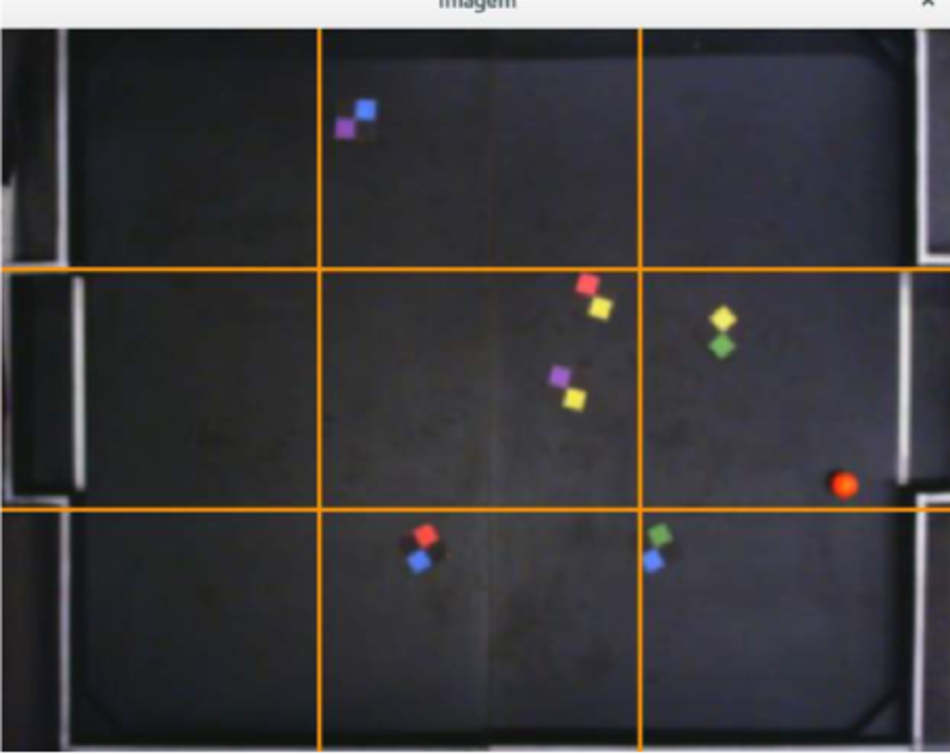
\includegraphics[width=0.4\textwidth]{vssvision.pdf} 	
	\caption{Sistema de calibracao desenvolvido peloSIRLab \cite{Rosa:2015}}
	\label{SIRLabCalibracao}
\end{figure}
Rosa menciona que a calibração de cores e feita calibrando obrigatoriamente laranja, amarelo e azul, e então as outras cores referentes aos jogadores em campo. Como visto na Figura \ref{SIRLabCalibracao} a imagem da c\^amera é dividida em nove cantos, e para calibrar a cor o usuário deve clicar em cima da cor que gostaria de ser calibrada, assim salvando um intervalo de cor tratado como RGB máximo e o mínimo daquela cor , a medida
que vão havendo os cliques o sistema verifica para cada atributo se ele é maior que o atributo
máximo salvo ou menor que mínimo salvo, caso seja, o mesmo assume o lugar de menor ou
maior\cite{Rosa:2015} e esse processo deve ser feito em cada um dos nove cantos da imagem. Os valores HSV encontrados s\~ao ajustados manualmente com a ajuda de sliders, como visto na Figura \ref{SIRLabCalibracaoHSV}. Este processo de calibração pode demorar entre cinco e dez minutos.
O desenvolvimento do sistema utiliza para processamento de imagens a biblioteca OpenCV e para telas interativas a biblioteca  ImGui.

\begin{figure}[!h]
	\centering
	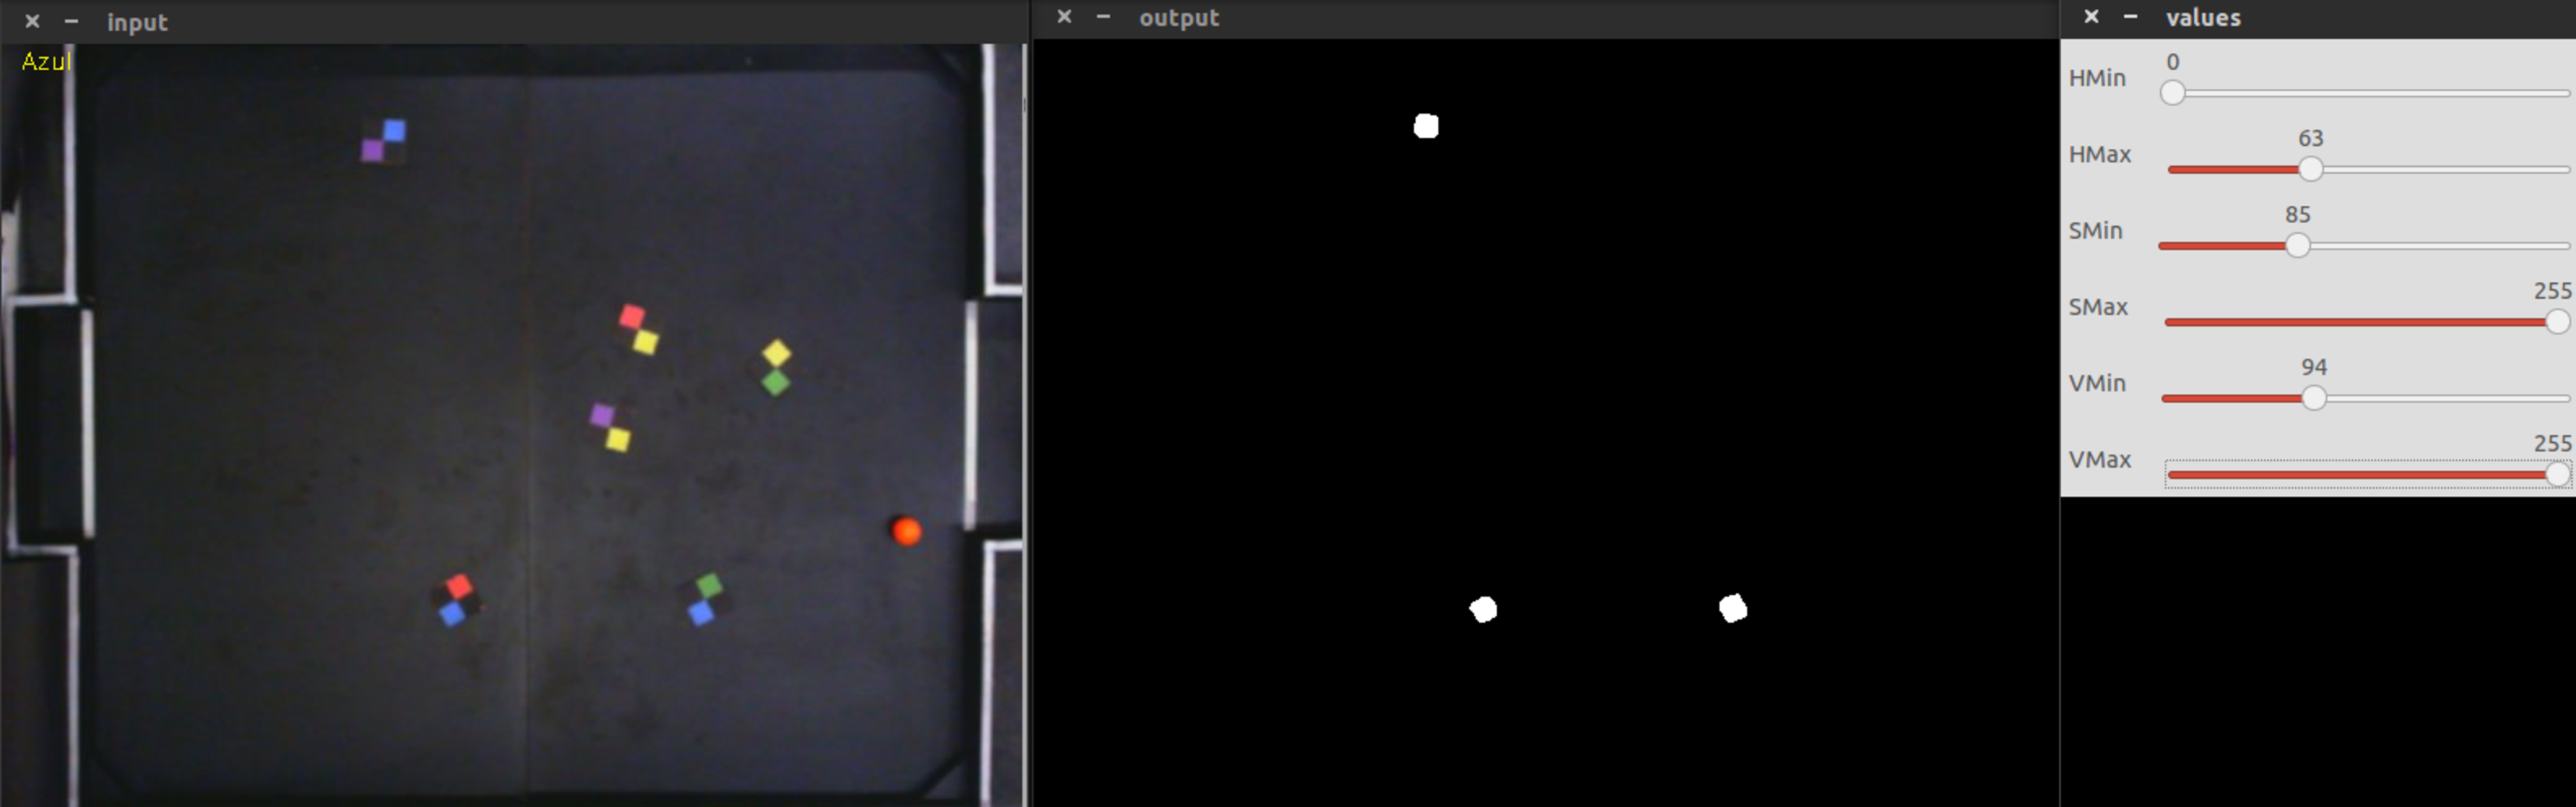
\includegraphics[width=0.8\textwidth]{calibration.pdf} 	
	\caption{Sistema de calibracao desenvolvido peloSIRLab \cite{VSSVision}}
	\label{SIRLabCalibracaoHSV}
\end{figure}

O atual sistema de visão computacional do SIRLab passou por algumas mudanças desde 2015 e conta com uma inteface e metodo de calibração diferentes\cite{VSSVision}. 

Como disponível no repositorio online do Laboratorio, o atual sistema de calibração de cores utiliza o espaço de cores HSV, no lugar do RGB\cite{Rosa:2015}. A antiga inteface do sistema, feita inicialmente em ImGui deu lugar a nova, desenvolvida em Qt, como mostra a Figura \ref{SIRLabNova}.

O método de calibração de cores também foi modificado, segundo a equipe\cite{VSSVision} o sistema possibilita a calibragem de 8 cores, Laranja, Amarelo, Azul, Vermelho, Verde, Rosa, Roxo, Marrom. Após o usuário escolher uma cor para calibrar o mesmo deve encontrar um intervalo de cor, no espaço de cores HSV, que represente-a. Ao clicar na tela com o botão direito o sistema da um zoom na área para ajuste fino. A Figura \ref{SIRLabNovaCalibracao} demonstra o novo método de calibração.
\begin{figure}[H]
\begin{minipage}[H]{0.45\linewidth}
\hspace{0.5cm}
\centering
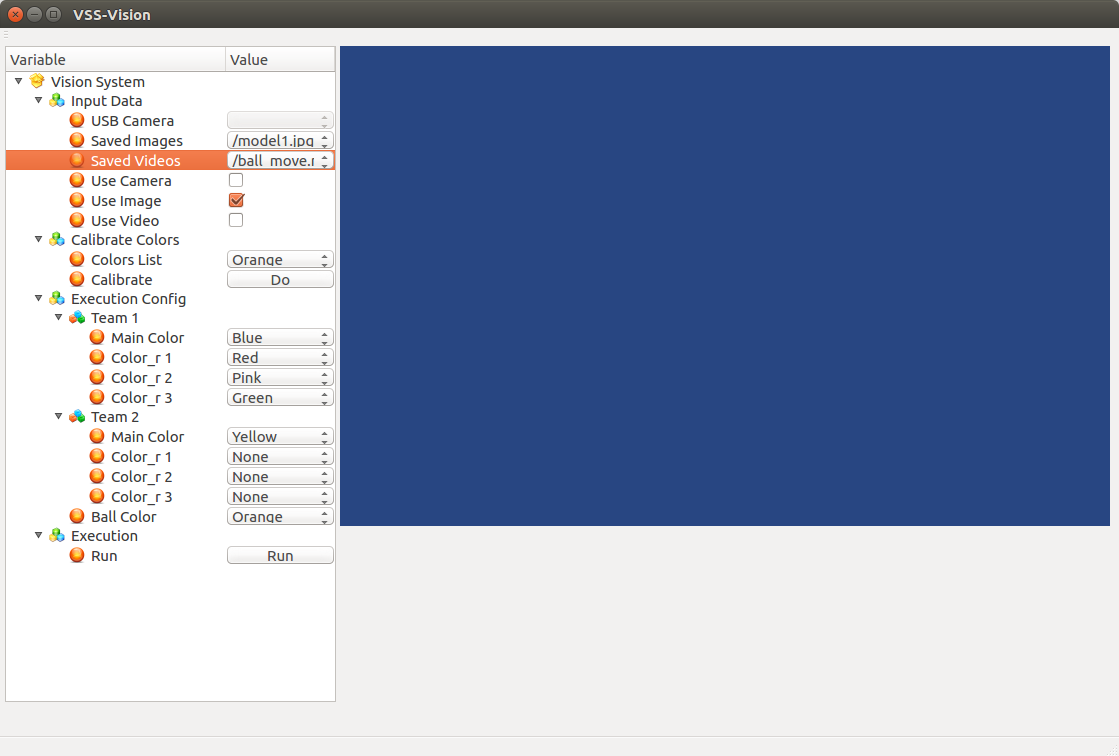
\includegraphics[width=\textwidth]{vsssnovonormal.png}
\caption{Nova interface do time da SIRLab \cite{VSSVision}}
\label{SIRLabNova}
\end{minipage}
\hspace{0.5cm}
\begin{minipage}[H]{0.40\linewidth}
\centering
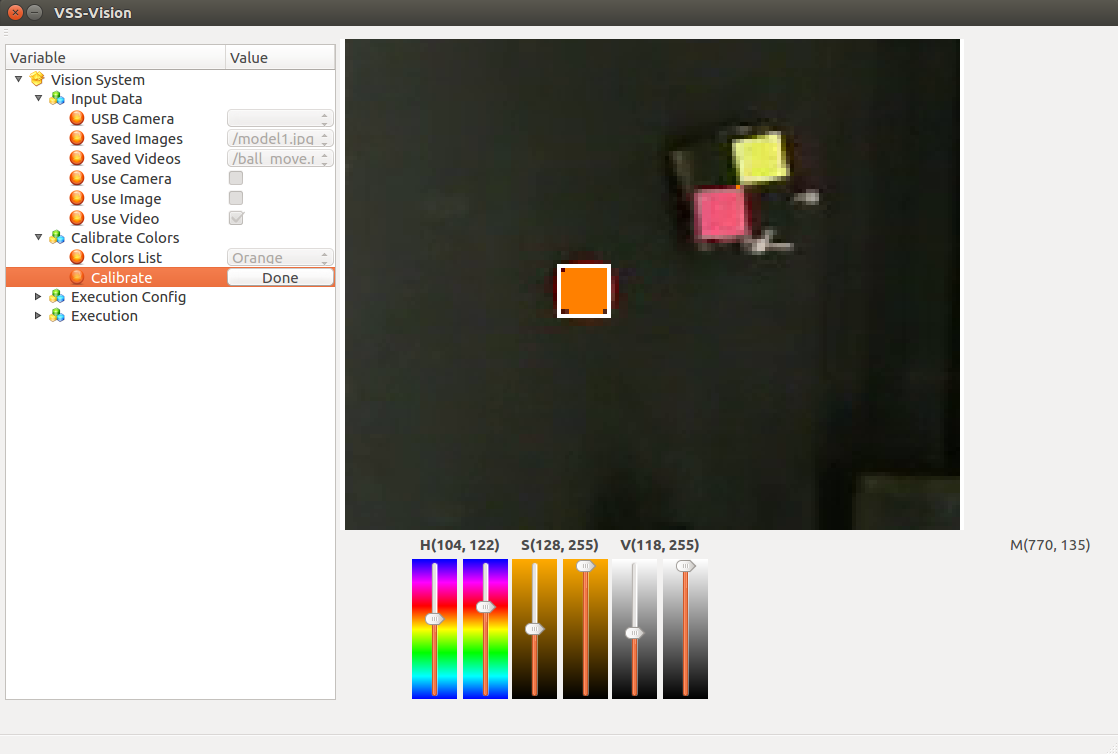
\includegraphics[width=\textwidth]{vsssnovo.png}
\caption{Calibração atual do time da SIRLab \cite{VSSVision} após calibração}
\label{SIRLabNovaCalibracao}
\end{minipage}
\end{figure}	


\section{Organização da Trabalho} \label{Sec:Organizacao}

Este trabalho está divido em cinco capítulos, incluindo esta introdução como capítulo inicial. No segundo capítulo encontra-se a fundamentação teórica do texto, contento informaç\~oes sobre processamento de imagens referente à detecção de objetos e cores. A descrição da probabilidade usada no trabalho, na descoberta do tamanho desejável dos objetos, uma breve descrição sobre o futebol de robôs. No terceiro capítulo encontra-se todo o desenvolvimento do projeto, suas classes, a descrição das tecnologias utilizadas no projeto, e o detalhamento de cada um dos tipos de calibração. No quarto capítulo são apresentados os testes e os resultados obtidos em cada um dos testes do projeto. No quinto capítulo são feitas as conclusões do trabalho e considerações finais, bem como expostas melhorias que possam vir a ser implementadas em trabalhos futuros.
